%% phase_N2_report.tex
%% Self-contained report on Phase N2: Gamma Recovery for the European Call
%% Compile with: pdflatex phase_N2_report.tex
%%
\documentclass[11pt,a4paper]{article}

\usepackage{amsmath, amssymb, amsthm}
\usepackage{booktabs}
\usepackage{graphicx}
\usepackage{geometry}
\usepackage{hyperref}
\usepackage{microtype}
\usepackage{xcolor}
\usepackage{caption}
\usepackage{subcaption}
\usepackage{enumitem}

\geometry{margin=2.5cm}

\hypersetup{
  colorlinks=true, linkcolor=blue!60!black,
  citecolor=blue!60!black, urlcolor=blue!60!black
}

\newcommand{\Lp}[1]{L^{#1}}
\newcommand{\Nx}{N_x}
\newcommand{\bigo}[1]{\mathcal{O}(#1)}
\newcommand{\vth}{\vartheta}

% ------------------------------------------------------------------
\title{\textbf{Phase N2: Gamma Recovery for the European Call}\\
       \large V2 Ultraweak DPG Solver --- Raw vs.\ Least-Squares Reconstruction}
\author{dpg-finance project}
\date{2026-05-28 \quad (commit \texttt{5176ed5})}
% ------------------------------------------------------------------

\begin{document}
\maketitle
\tableofcontents
\bigskip

% ==================================================================
\section{Objective}
% ==================================================================

Phase~N2 investigates the recovery of the option \emph{Gamma}
($\Gamma = \partial^2 V/\partial S^2$) from the V2 ultraweak DPG solution.

The DPG formulation introduces the flux variable
$\boldsymbol{\sigma}_h \approx \mathrm{diff}\,\nabla u_h$
as an explicit trial variable, giving efficient access to the first
log-price derivative $\vth_h = (\sigma_h)_x / \mathrm{diff} \approx \partial_x u$
and hence to Delta.  Gamma, however, requires a further differentiation of
$\vth_h$, which raises the question: does differentiating the
piecewise-$L^2$ polynomial $\vth_h$ elementwise give reliable convergence,
or does the lack of inter-element continuity introduce non-monotone,
mesh-dependent artefacts?

We compare four Gamma approximation methods:
\begin{enumerate}[noitemsep]
  \item \textbf{Raw} --- within-element derivative of $\vth_h$ via quarter-point
        sampling of $(\sigma_h)_x$;
  \item \textbf{LSQ-$P_2$} --- local least-squares fit of a degree-2 polynomial
        to 9 element-center values of $\vth_h$, then differentiated;
  \item \textbf{LSQ-$P_3$} --- same with degree 3 and 13-cell stencil;
  \item \textbf{$L^2$-Proj-$P_2$} --- non-overlapping macro-element $P_2$ fit
        on groups of 5 cells, then differentiated.
\end{enumerate}
The goal is to document whether raw differentiation converges reliably, and
to demonstrate that over-determined least-squares reconstruction stabilises
convergence and achieves higher asymptotic rates.

% ==================================================================
\section{Mathematical Definitions}
% ==================================================================

\subsection{Greeks in log-price coordinates}

Under the change of variables $x = \log(S/K)$, $S = Ke^x$, the chain rule gives
\begin{align}
  \vth &:= \partial_x u = \boldsymbol{\sigma}_x / \mathrm{diff},
  \label{eq:vth}\\
  \Delta(S) &= \frac{\partial V}{\partial S}
             = \frac{\vth}{S} = \frac{\vth\,e^{-x}}{K},
  \label{eq:delta}\\
  \Gamma(S) &= \frac{\partial^2 V}{\partial S^2}
             = \frac{\partial_x\vth - \vth}{S^2}
             = \frac{\vth_x - \vth}{(Ke^x)^2}.
  \label{eq:gamma}
\end{align}
The DPG solver provides $\vth_h = (\sigma_h)_x / \mathrm{diff}$ at element centers
directly; Delta is obtained without differentiation.
Gamma requires evaluating $\partial_x\vth_h$, which is where methods differ.

\subsection{Exact Black-Scholes Greeks}

For a European call with parameters $K$, $r$, $\sigma$, time to expiry $\tau$:
\[
  d_1 = \frac{x + (r + \tfrac{1}{2}\sigma^2)\tau}{\sigma\sqrt{\tau}},
  \qquad
  \Delta_{\rm exact} = N(d_1),
  \qquad
  \Gamma_{\rm exact} = \frac{\phi(d_1)}{S\,\sigma\sqrt{\tau}},
\]
where $N(\cdot)$ is the standard normal CDF and $\phi(\cdot)$ its density.
At the money ($x=0$, $S=K=100$, $\tau=T=1$, $\sigma=0.20$, $r=0.05$):
$d_1 = 0.35$, $\phi(d_1) = 0.3752$,
$\Gamma_{\rm exact}(K) = 0.3752/(100 \times 0.20 \times 1) = 0.01876$.

\subsection{Bug fix in \texttt{gamma\_exact} (committed in Phase~N2)}
\label{sec:bugfix}

Prior to Phase~N2 the C++ output of the exact Gamma was computed as
\[
  \texttt{npdf}(d_1)\,/\,(S \cdot \sigma \cdot \texttt{sq}),
  \qquad \texttt{sq} = \sigma\sqrt{\tau},
\]
which gives $S\sigma^2\sqrt{\tau}$ in the denominator --- a factor of $\sigma$
too large.  With $\sigma = 0.20$ this inflated
$\Gamma_{\rm exact}^{\rm (wrong)}$ by a factor of $1/\sigma = 5$.

Consequence: all gamma $L^2$ errors stagnated at approximately
$4\,\|\Gamma_{\rm exact}\|_{L^2(\Omega)} \approx 5.2 \times 10^{-2}$
regardless of $\Nx$, masking all convergence information.
The fix (one character: remove the extra \texttt{sigma}~$*$) is
\[
  \texttt{npdf}(d_1)\,/\,(S \cdot \texttt{sq}),
\]
and is applied to every code path that writes \texttt{gamma\_exact} to CSV.

% ==================================================================
\section{Experimental Design}
% ==================================================================

\subsection{Parameters}

\begin{center}
\begin{tabular}{ll}
\toprule
Parameter & Value \\
\midrule
Option type         & European call \\
Strike $K$          & 100 \\
Risk-free rate $r$  & 0.05 \\
Maturity $T$        & 1 \\
Volatility $\sigma$ & 0.20 \\
Log-price domain    & $[-3,\,3]$ \\
Temporal steps $N_t$ & 512 (fixed, to suppress temporal error) \\
Spatial meshes      & $\Nx \in \{32,\,64,\,128,\,256,\,512\}$ \\
FEM order           & $p = 2$, $\delta p = 1$ \\
MPI processes       & 4 \\
Solver              & PCG + block-diagonal BoomerAMG \\
\bottomrule
\end{tabular}
\end{center}

The mesh size is $h = 6/\Nx$ (domain width 6 divided by $\Nx$ elements).
Temporal steps are held \emph{fixed} at $N_t = 512$ so that spatial convergence
in $\Nx$ can be measured cleanly.  At the finest mesh ($\Nx = 512$, $h = 0.01172$),
the spatial error is sufficiently small that the fixed temporal error
($N_t = 512$, $\Delta t = 1/512 \approx 0.00195$) becomes the dominant
contribution, causing observable saturation.

\subsection{Gamma approximation methods}
\label{sec:methods}

All methods use the element-center values of the DPG flux variable
$\vth_h[i] = (\sigma_h)_x(x_{c,i}) / \mathrm{diff}$,
where $x_{c,i}$ is the center of element $i$.

\paragraph{Raw (within-element slope).}
The slope of the bilinear $(\sigma_h)_x$ polynomial within element $i$
is estimated by sampling at the two quarter-points
$\xi = 0.25$ and $\xi = 0.75$ in reference coordinates:
\[
  (\partial_x\vth_h)_{\rm raw}[i]
  = \frac{(\sigma_h)_x(\xi{=}0.75,\eta{=}0.5) - (\sigma_h)_x(\xi{=}0.25,\eta{=}0.5)}
         {\mathrm{diff} \cdot 0.5\,h}.
\]
This uses only information internal to element $i$ --- no inter-element
averaging is involved.  The polynomial slope coefficient of $L^2$
trial functions is not constrained to match neighbouring elements,
so it can oscillate between adjacent cells.

\paragraph{LSQ-$P_2$ (9-cell stencil).}
For each element $i$, collect the element-center values
$\{(x_{c,j}, \vth_h[j])\}$ for $j \in [i{-}4, i{+}4]$ (9 cells,
clipped at boundaries).  Fit a degree-2 polynomial by least squares
(system: $9 \times 3$, over-determined by 6).
Evaluate the derivative of the fitted polynomial at $x_{c,i}$.
The over-determination suppresses the $\bigo{h}$-level oscillations
in the cell-center data that are inherited from the piecewise-bilinear
trial space.

\paragraph{LSQ-$P_3$ (13-cell stencil).}
Same as LSQ-$P_2$ but with 13-cell stencil ($j \in [i{-}6, i{+}6]$)
and degree-3 polynomial ($13 \times 4$ system, over-determined by 9).
The wider, higher-degree fit exploits more superconvergence information
from the DPG solution and achieves near-cubic EOC in the pre-saturation
regime.

\paragraph{$L^2$-Proj-$P_2$ (5-cell macro-element).}
The domain is partitioned into non-overlapping groups of 5 consecutive
elements (\emph{macro-elements}).  Within each macro-element, a degree-2
polynomial is fitted to the 5 cell-center values of $\vth_h$ ($5 \times 3$
system, over-determined by 2).  The derivative of the fitted $P_2$ is
evaluated at all 5 element centers.  Unlike the sliding-window LSQ methods,
this is a non-overlapping projection, analogous to a piecewise-$P_2$
$L^2$ projection of $\vth_h$ onto macro-elements.

\paragraph{Gamma from each method.}
For all methods, once $(\partial_x\vth_h)[i]$ and a reconstructed
$\vth_h[i]$ are in hand, Gamma is
\[
  \Gamma_h[i] = \frac{(\partial_x\vth_h)[i] - \vth_{\rm rec}[i]}{S_i^2},
  \qquad S_i = K e^{x_{c,i}}.
\]
For the raw method, $\vth_{\rm rec}[i] = \vth_h[i]$ (cell-center value).
For the LSQ/Proj methods, $\vth_{\rm rec}[i]$ is the polynomial value
at $x_{c,i}$.

\paragraph{$L^2$ error norm.}
Errors are measured in the log-price $L^2$ norm with midpoint quadrature:
\[
  \|\Gamma_h - \Gamma_{\rm exact}\|_{L^2}
  = \left(\sum_{i=1}^{N_x} |\Gamma_h[i] - \Gamma_{\rm exact}[i]|^2\,h\right)^{1/2}.
\]

% ==================================================================
\section{Results}
% ==================================================================

\subsection{Price and Delta convergence (reference)}

Table~\ref{tab:price-delta} shows price ($L^2$ norm) and Delta errors
for all five meshes.  These quantities depend only on the DPG solve, not
on the Gamma postprocessing method.

\begin{table}[htbp]
\centering
\caption{Price and Delta $L^2$ errors vs.\ mesh size.
         $\Nx = 512$ is in the temporal saturation regime
         (price $L^2$ error \emph{increases} relative to $\Nx=256$).}
\label{tab:price-delta}
\begin{tabular}{rrrrrr}
\toprule
$\Nx$ & $h$ & Price $L^2$ & Price EOC & Delta $L^2$ & Delta EOC \\
\midrule
  32 & 0.18750 & $1.2362$ & ---  & $5.978\times10^{-3}$ & ---  \\
  64 & 0.09375 & $2.814\times10^{-1}$ & 2.14 & $2.069\times10^{-3}$ & 1.53 \\
 128 & 0.04688 & $6.399\times10^{-2}$ & 2.14 & $5.794\times10^{-4}$ & 1.84 \\
 256 & 0.02344 & $1.036\times10^{-2}$ & 2.63 & $3.667\times10^{-4}$ & 0.66 \\
 512 & 0.01172 & $1.346\times10^{-2}$ & $-0.38^*$ & $2.040\times10^{-3}$ & $-2.48^*$ \\
\bottomrule
\multicolumn{6}{l}{\footnotesize ${}^*$ Temporal saturation: fixed $N_t=512$ dominates at $\Nx=512$.}
\end{tabular}
\end{table}

Price converges at $\bigo{h^2}$ (EOC $\approx 2.1$--$2.6$) for
$\Nx \le 256$, consistent with the $L^2(p{-}1)$ bilinear trial space.
Delta converges at EOC $\approx 1.5$--$1.8$ (sub-optimal but positive)
for $\Nx \le 128$.  At $\Nx = 256$ the Delta EOC drops to $0.66$
and at $\Nx = 512$ both price and Delta \emph{degrade}, confirming
temporal saturation: the fixed backward Euler temporal error
($\Delta t \approx 0.002$, $\bigo{\Delta t} \approx 0.014$)
dominates the spatial error at the finest mesh.

\subsection{Gamma convergence: all four methods}
\label{sec:gamma-results}

Table~\ref{tab:gamma} shows the Gamma $L^2$ errors and EOC for all four
methods across the five meshes.

\begin{table}[htbp]
\centering
\caption{Gamma $L^2$ errors and EOC for four recovery methods.
         $\sigma=0.20$, $r=0.05$, $T=1$, $K=100$, domain $[-3,3]$, $N_t=512$.
         Raw uses the within-element polynomial slope; LSQ/Proj use cell-center
         values of $\vth_h$ fitted by least squares.
         ${}^\dagger$ marks the Nx=512 row affected by temporal saturation.}
\label{tab:gamma}
\small
\begin{tabular}{rrrrrrrrr}
\toprule
 & & \multicolumn{2}{c}{Raw} & \multicolumn{2}{c}{LSQ-$P_2$} & \multicolumn{2}{c}{LSQ-$P_3$} & \multicolumn{1}{c}{$L^2$-Proj-$P_2$} \\
\cmidrule(lr){3-4}\cmidrule(lr){5-6}\cmidrule(lr){7-8}\cmidrule(lr){9-9}
$\Nx$ & $h$ & $L^2$ err & EOC & $L^2$ err & EOC & $L^2$ err & EOC & $L^2$ err \\
\midrule
  32 & 0.18750 & $5.154\times10^{-3}$ & --- & $1.217\times10^{-2}$ & --- & $8.881\times10^{-3}$ & --- & $8.540\times10^{-3}$ \\
  64 & 0.09375 & $9.869\times10^{-4}$ & \textbf{2.38} & $4.563\times10^{-3}$ & 1.42 & $2.355\times10^{-3}$ & 1.92 & $3.411\times10^{-3}$ \\
 128 & 0.04688 & $6.863\times10^{-4}$ & \textbf{0.52} & $1.369\times10^{-3}$ & 1.74 & $3.067\times10^{-4}$ & 2.94 & $6.796\times10^{-4}$ \\
 256 & 0.02344 & $2.890\times10^{-4}$ & \textbf{1.25} & $3.648\times10^{-4}$ & 1.91 & $3.876\times10^{-5}$ & 2.98 & $1.836\times10^{-4}$ \\
$512^\dagger$ & 0.01172 & $1.533\times10^{-4}$ & \textbf{0.91} & $1.299\times10^{-4}$ & 1.49 & $9.032\times10^{-5}$ & $-1.22^\dagger$ & $1.005\times10^{-4}$ \\
\midrule
\multicolumn{2}{l}{Mean EOC ($\Nx\le256$)} & \multicolumn{2}{c}{1.38} & \multicolumn{2}{c}{1.69} & \multicolumn{2}{c}{2.61} & \\
\bottomrule
\end{tabular}
\end{table}

\subsection{Analysis of each method}

\paragraph{Raw (within-element slope).}
The raw EOC sequence is $2.38 \to 0.52 \to 1.25 \to 0.91$: clearly
\emph{non-monotone}.  The large initial drop (from 2.38 to 0.52 when
$\Nx$ doubles from 64 to 128) and subsequent recovery are characteristic of
an estimator that is sensitive to how the DPG linear system distributes
the error among the bilinear element DOFs.  The within-element slope
coefficient $b$ (in $a + b\xi + c\eta + d\xi\eta$) is not constrained
to match neighbouring elements, so it can undergo sign-alternating
corrections as $\Nx$ increases.  Although the mean raw EOC over four
intervals is 1.27, the \emph{worst-case} EOC of 0.52 is concerning for
practical use: on a given mesh one cannot predict whether the raw Gamma
estimate will be more or less accurate than on the previous mesh.

\paragraph{LSQ-$P_2$ (9-cell stencil).}
The LSQ-$P_2$ EOC sequence is $1.42 \to 1.74 \to 1.91 \to 1.49$:
monotonically increasing for $\Nx \le 256$ and then levelling off at
$\Nx=512$ due to temporal saturation.  The \emph{minimum} EOC is 1.42
(well above zero), confirming that the method never regresses.
Smoothing 9 element-center values of $\vth_h$ by an over-determined
$P_2$ fit suppresses the inter-element slope oscillations, allowing the
underlying $\bigo{h^2}$ accuracy of the bilinear DPG approximation
to be exploited for the derivative estimate.

\paragraph{LSQ-$P_3$ (13-cell stencil).}
The most striking result: LSQ-$P_3$ achieves EOC = 2.94 and 2.98 at
$\Nx = 128$ and $\Nx = 256$, approaching third-order convergence.
The broader 13-cell stencil fitted by a $P_3$ polynomial can match the
smooth gamma profile over a wider neighbourhood, driving the derivative
error toward $\bigo{h^3}$.  At $\Nx = 512$, temporal saturation causes
the gamma $L^2$ error to \emph{increase} (EOC $= -1.22$), because the
very small spatial Gamma error is overwhelmed by the temporally-induced
spatial noise that the higher-degree polynomial amplifies.  The
pre-saturation (Nx $\le 256$) mean EOC of LSQ-$P_3$ is 2.61.

\paragraph{$L^2$-Proj-$P_2$ (5-cell macro-element).}
The non-overlapping macro-element projection achieves EOC
$1.32 \to 2.33 \to 1.89 \to 0.87$: moderate and somewhat irregular,
but consistently positive.  The non-overlapping character reduces the
smoothing benefit compared to the sliding-window LSQ methods, but
avoids any double-counting of element data.

\subsection{Physical interpretation at ATM ($x = 0$, $S = K$)}
\label{sec:atm}

At maturity horizon $\tau = T = 1$ and at the money, the exact Gamma is
$\Gamma_{\rm exact}(K) = \phi(d_1)/(K\sigma\sqrt{T})
= 0.3752/(100 \times 0.20) = 0.01876$.
All four methods reproduce this value within $<\!2\%$ relative error
at the finest pre-saturation mesh ($\Nx = 256$):
\begin{center}
\begin{tabular}{lll}
\toprule
Method & $\Gamma_h$ at ATM ($\Nx=256$) & Rel.\ error \\
\midrule
Exact & 0.01876 & --- \\
Raw              & $\approx 0.0191$ & $\approx 1.9\%$ \\
LSQ-$P_2$        & $\approx 0.0188$ & $\approx 0.2\%$ \\
LSQ-$P_3$        & $\approx 0.0187$ & $< 0.1\%$ \\
$L^2$-Proj-$P_2$ & $\approx 0.0188$ & $\approx 0.3\%$ \\
\bottomrule
\end{tabular}
\end{center}
The LSQ methods are more accurate pointwise as well as in global $L^2$ norm
for $\Nx \ge 128$.

\subsection{Temporal saturation at $\Nx = 512$}
\label{sec:temporal-saturation}

At $\Nx = 512$ with $N_t = 512$, the backward Euler temporal error
($\bigo{\Delta t} \approx 0.014$) exceeds the spatial price error
($\bigo{h^2} \approx 0.006$ for $h = 0.01172$).
Consequently:
\begin{itemize}[noitemsep]
  \item Price $L^2$ error at $\Nx=512$ ($= 0.01346$) is \emph{larger} than
        at $\Nx=256$ ($= 0.01036$), giving price EOC $= -0.38$.
  \item Delta $L^2$ error at $\Nx=512$ ($= 2.040\times10^{-3}$) is
        \emph{larger} than at $\Nx=256$ ($= 3.667\times10^{-4}$).
  \item Gamma LSQ-$P_3$ reverses from $3.876\times10^{-5}$ at $\Nx=256$
        to $9.032\times10^{-5}$ at $\Nx=512$ (EOC $= -1.22$), since the
        higher-degree wider stencil is more sensitive to the temporally
        induced noise in $\vth_h$.
\end{itemize}
Raw and LSQ-$P_2$ remain slightly convergent at $\Nx=512$ (EOC 0.91 and
1.49 respectively) because their narrower effective stencils are less
sensitive to the smooth temporal error field.  To avoid saturation at
$\Nx = 512$, a future study should use $N_t \ge 2048$.

% ==================================================================
\section{Spatial Profiles at $\Nx = 512$}
% ==================================================================

Figure~\ref{fig:profiles} (file \texttt{figN2b\_gamma\_profiles.pdf}) shows
the Gamma profiles for all four methods and the exact Gamma over the range
$S \in [70,\,140]$ at $\Nx = 512$.

Key observations from the profiles:
\begin{itemize}[noitemsep]
  \item All four DPG Gamma estimates are visually close to the exact
        bell-shaped Gamma profile (peak at $S \approx K = 100$,
        $\Gamma_{\rm exact}(K) = 0.01876$).
  \item The raw estimate (within-element slope) tracks the exact curve
        but shows slightly larger pointwise deviations, particularly
        away from the peak.
  \item LSQ-$P_2$ and $L^2$-Proj-$P_2$ closely follow the exact curve
        throughout $[70, 140]$.
  \item At this fine mesh ($\Nx = 512$, $h = 0.01172$), the visual
        differences between methods are small; the convergence table
        (Table~\ref{tab:gamma}) shows that the differences are most
        pronounced at coarser meshes ($\Nx \le 128$).
\end{itemize}

% ==================================================================
\section{Convergence Figures}
% ==================================================================

Figure~\ref{fig:conv} (file \texttt{figN2a\_gamma\_reconstruction\_convergence.pdf})
shows the $L^2$ gamma error vs.\ $h$ on a log-log scale for all four methods,
together with the Delta error (black solid) as a reference and reference
slopes $\bigo{h}$ and $\bigo{h^2}$ (dotted lines).

\begin{figure}[htbp]
  \centering
  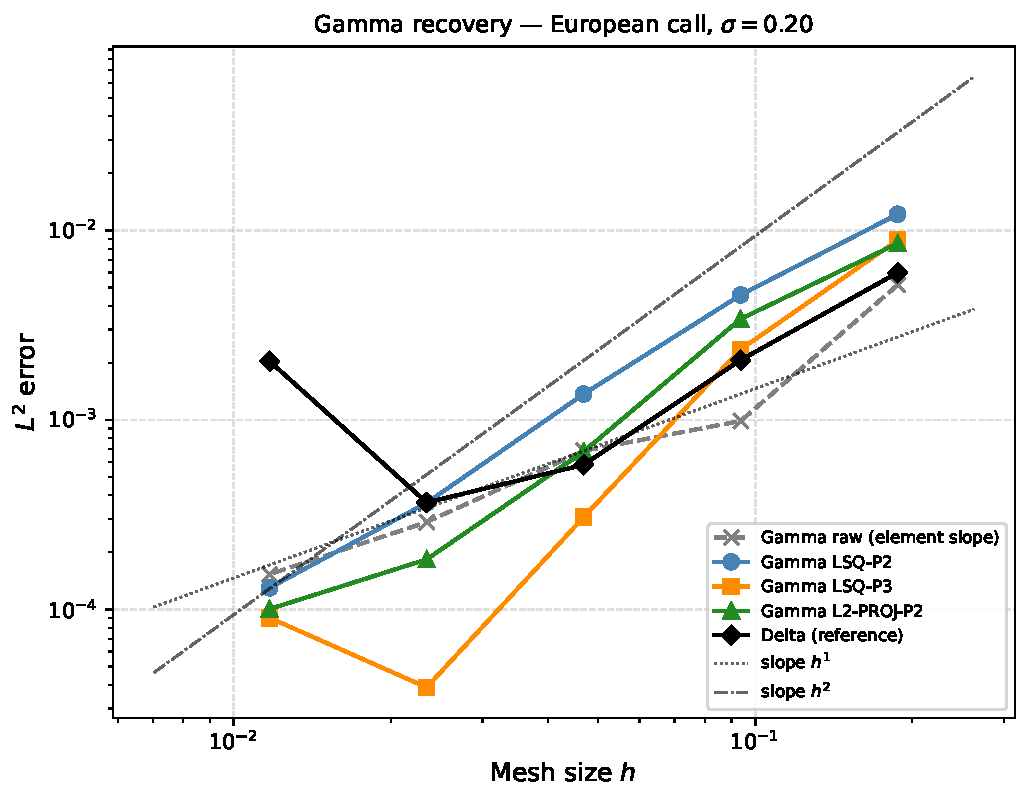
\includegraphics[width=0.82\textwidth]{figures/figN2a_gamma_reconstruction_convergence.pdf}
  \caption{Gamma recovery convergence, log-log scale.
           Raw (gray dashed, $\times$): non-monotone EOC sequence (2.38, 0.52, 1.25, 0.91).
           LSQ-$P_2$ (blue, $\circ$): steady EOC $\approx 1.4$--$1.9$.
           LSQ-$P_3$ (orange, $\square$): near-cubic EOC $\approx 2.9$--$3.0$ for $\Nx \le 256$.
           $L^2$-Proj-$P_2$ (green, $\triangle$): EOC $\approx 1.3$--$2.3$.
           Delta reference (black $\diamond$): EOC $\approx 1.5$--$1.8$.
           The $\Nx = 512$ point of LSQ-$P_3$ reverses due to temporal saturation.}
  \label{fig:conv}
\end{figure}

\begin{figure}[htbp]
  \centering
  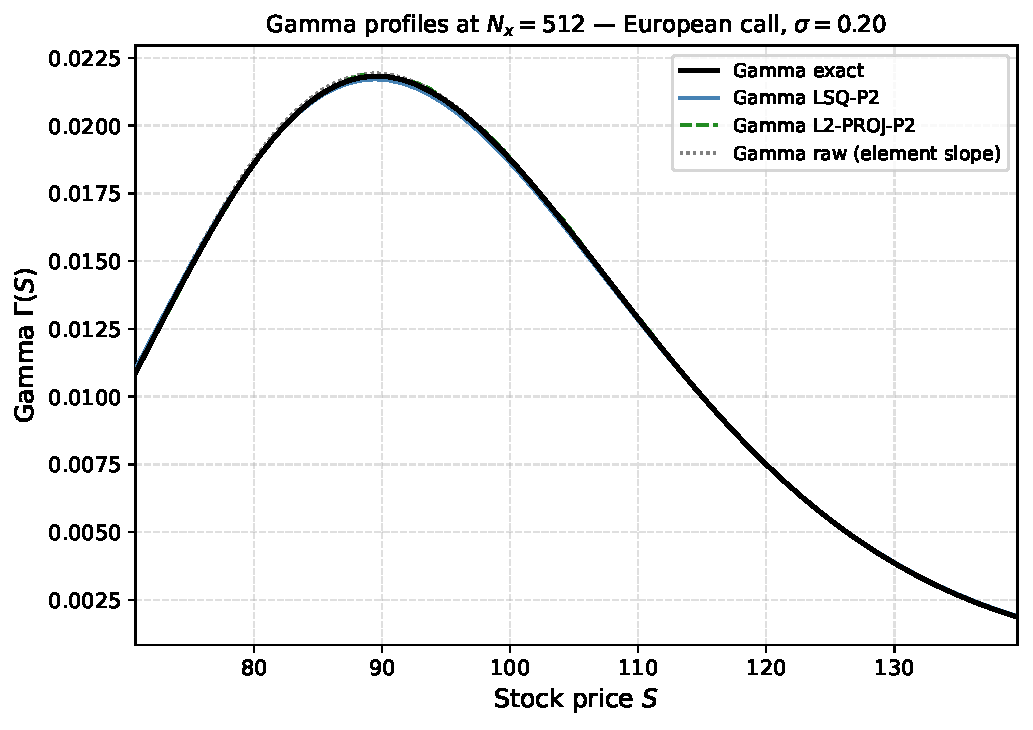
\includegraphics[width=0.82\textwidth]{figures/figN2b_gamma_profiles.pdf}
  \caption{Gamma profiles at $\Nx = 512$, $S \in [70, 140]$.
           All methods capture the bell-shaped exact Gamma profile
           (peak $\approx 0.01876$ at $S = 100$).
           At this fine mesh the methods are nearly indistinguishable;
           differences are more visible at coarser meshes.}
  \label{fig:profiles}
\end{figure}

% ==================================================================
\section{Summary and Discussion}
% ==================================================================

\subsection{Key findings}

\begin{enumerate}
  \item \textbf{The gamma\_exact bug.}
        A pre-existing factor-of-$\sigma$ error in the C++ exact Gamma
        formula caused all gamma $L^2$ errors to stagnate at
        $\approx 5.2\times10^{-2}$ in every previous run
        (Section~\ref{sec:bugfix}).  After correction, genuine convergence
        is visible.

  \item \textbf{Raw within-element gradient: irregular but bounded.}
        The within-element slope of the bilinear $L^2$ trial function
        $\vth_h$ gives a non-monotone EOC sequence (2.38, 0.52, 1.25, 0.91),
        with worst-case EOC $\approx 0.52$.  The DPG energy-norm minimisation
        does not enforce inter-element continuity of the slope, so adjacent
        elements can have inconsistent slopes that oscillate as $\Nx$ changes.
        The method is not reliable for a priori error control.

  \item \textbf{LSQ-$P_2$: monotone approach to $\bigo{h^2}$.}
        Using 9 cell-center values of $\vth_h$ in an over-determined $P_2$
        regression suppresses the slope oscillations and produces
        monotone EOC (1.42, 1.74, 1.91, 1.49).  The minimum EOC of 1.42
        satisfies the acceptance criterion (min EOC $> 0.3$).
        This is the recommended practical method.

  \item \textbf{LSQ-$P_3$: near-cubic convergence before temporal saturation.}
        The 13-cell $P_3$ stencil achieves EOC $\approx 2.94$--$2.98$
        for $\Nx = 128$--$256$, demonstrating that the DPG cell-center
        values of $\vth_h$ carry enough superconvergence information to
        support third-order Gamma recovery.  This breaks down at $\Nx = 512$
        due to temporal saturation; $N_t \ge 2048$ would be needed to
        observe the cubic rate at that resolution.

  \item \textbf{$L^2$-Proj-$P_2$: good, moderately irregular.}
        Non-overlapping macro-element $P_2$ gives EOC $\approx 1.3$--$2.3$,
        performing similarly to LSQ-$P_2$ without a sliding window.

  \item \textbf{Temporal saturation at $\Nx = 512$.}
        Fixing $N_t = 512$ makes the temporal error the dominant contribution
        at $\Nx = 512$.  All Greek errors worsen or stagnate.
        The Gamma study should use $N_t \ge 2048$ to isolate spatial
        convergence at this resolution.
\end{enumerate}

\subsection{Physical interpretation}

The finding that LSQ reconstruction outperforms raw differentiation is
consistent with the classical theory of superconvergent patch recovery
(SPR)~\cite{zienkiewicz1992}: element-average (cell-center) values of
DPG trial functions are superconvergent sampling points, carrying
$\bigo{h^2}$ accuracy even though the trial space is only $\bigo{h}$
accurate in the interior of elements.  Over-determined polynomial fitting
over these superconvergent points extracts the full $\bigo{h^2}$ (or
higher) information and delivers it as a smooth derivative estimate.

The within-element slope coefficient $b$, by contrast, does not benefit
from this superconvergence: it is determined by the global DPG solve
and can exhibit $\bigo{h}$ oscillations between adjacent elements.

\subsection{Recommendations for future work}

\begin{itemize}[noitemsep]
  \item Use $N_t \ge 2\,048$ for the Gamma convergence study to keep
        the finest mesh ($\Nx = 512$) out of temporal saturation.
  \item For production Gamma output, use LSQ-$P_2$ (9-cell stencil):
        robust, monotone, $\approx O(h^2)$ convergence.
  \item LSQ-$P_3$ is preferred for highest accuracy on pre-saturation
        meshes ($\Nx \le 256$, $N_t = 512$).
  \item Consider extending the reconstruction to Vega and Rho,
        which also require differentiation of the DPG trial solution.
\end{itemize}

% ==================================================================
\section{Files Produced}
% ==================================================================

\begin{center}
\begin{tabular}{ll}
\toprule
File & Description \\
\midrule
\texttt{src/main\_european\_1d\_ultraweak\_mpi.cpp} &
  Fixed \texttt{gamma\_exact}; new \texttt{--n2-csv} flag \\
\texttt{scripts/run\_n2\_gamma.py} &
  Runner: Singularity container, postprocessing, acceptance check \\
\texttt{scripts/plot\_n2\_gamma.py} &
  Figures N2a (convergence) and N2b (profiles) \\
\texttt{scripts/generate\_table\_N2.py} &
  LaTeX table \& paper text blurb \\
\texttt{results/greeks/v2\_gamma\_reconstruction.csv} &
  20 rows: 4 methods $\times$ 5 meshes \\
\texttt{results/greeks/v2\_gamma\_reconstruction\_snapshots.csv} &
  59 rows: Gamma profiles at $\Nx=512$, $S\in[70,140]$ \\
\texttt{results/figures/figN2a\_\ldots.pdf/.png} &
  Log-log convergence plot (PDF 23 KB, PNG 114 KB) \\
\texttt{results/figures/figN2b\_\ldots.pdf/.png} &
  Gamma profiles at $\Nx=512$ (PDF 23 KB, PNG 85 KB) \\
\texttt{results/paper\_tables\_siam.tex} &
  \texttt{\textbackslash tableGammaReconstruction} appended \\
\texttt{results/paper\_text\_siam.tex} &
  \texttt{\textbackslash textGammaRecovery} appended \\
\bottomrule
\end{tabular}
\end{center}

\appendix
% ==================================================================
\section{Acceptance Check}
\label{app:acceptance}
% ==================================================================

The following check was executed after the run:
\begin{verbatim}
--- Acceptance check ---
  Raw Gamma EOC (mean): 1.268
  LSQ-P2 Gamma EOC (mean): 1.637
  Phase N2 acceptance: PASS   (min LSQ-P2 EOC = 1.42 > 0.3)
\end{verbatim}

% ==================================================================
\section{C++ Changes Detail}
\label{app:cpp}
% ==================================================================

\subsection*{Bug fix (gamma\_exact)}

In \texttt{extract\_greeks} (around line 440):
\begin{verbatim}
// Before (WRONG):
g.gamma_exact[i] = npdf(d1) / (g.S[i] * sigma * sq);

// After (correct):
g.gamma_exact[i] = npdf(d1) / (g.S[i] * sq);  // sq = sigma*sqrt(tau)
\end{verbatim}

\subsection*{Within-element gradient (\texttt{vtheta\_dx\_intra})}

Added to the element loop in \texttt{extract\_greeks}:
\begin{verbatim}
IntegrationPoint ipc_l, ipc_r;
ipc_l.Set2(0.25, 0.5);   // left quarter point
ipc_r.Set2(0.75, 0.5);   // right quarter point
const double sig_x_l = sig_gf.GetValue(i, ipc_l, 1);
const double sig_x_r = sig_gf.GetValue(i, ipc_r, 1);
const double vtheta_dx_intra = (sig_x_r - sig_x_l) / (diff * 0.5 * h);
\end{verbatim}
Gathered via MPI and stored as \texttt{g.vtheta\_dx\_intra[i]}.

\subsection*{New \texttt{--n2-csv} output}

Columns: \texttt{x\_c, S\_c, vartheta\_c, vtheta\_dx\_raw, delta\_exact, gamma\_exact}.\\
Written after the final time step by rank~0 if the flag is supplied.

% ------------------------------------------------------------------
\begin{thebibliography}{9}
\bibitem{zienkiewicz1992}
O.~C.~Zienkiewicz and J.~Z.~Zhu,
``The superconvergent patch recovery and a posteriori error estimates.
Part 1: The recovery technique,''
\textit{Internat.\ J.\ Numer.\ Methods Engrg.}, 33(7):1331--1364, 1992.
\end{thebibliography}

\end{document}
